\chapter{Methods}\label{cha:methods}

In this chapter, the selected methods for the experiments are presented and discussed.  
An understanding of the theoretical groundwork of the project from \Cref{cha:background} is assumed. A substantial part of the methods are taken directly or indirectly from the source code of Gasse et al. (2019) \cite{gasse2019exact}, Gupta et al. (2020) \cite{gupta2020hybrid} and the \gls{Ecole} source code \cite{prouvost2020ecole}. Some sentences and formulations are adapted from the project report \textit{Multi-layer Perceptrons for Branching in Mixed-Integer Linear Programming} (2020), as this thesis shares methods with the aforementioned report. 


\section{Dataset}\label{sec:dataset}

This section presents the selected data set and the process of generating trainable and testable data for the models. 
This will include a presentation of the problem instances, the generation of the expert solutions as well as the features that will be the input of the \gls{ML} models. 



\subsection{Problem Instances}\label{ssec:probleminstances}

In order to evaluate the methods presented in this project to the previous advances in the field, artificially generated \gls{MILP} problems found in Gasse et al. (2019) \cite{gasse2019exact} are used to train and evaluate the models. These problems are also the standard implemented in \gls{Ecole}.
The problems are expressed as pure binary programs. The results of the algorithm are, however, generalizable to general \gls{MILP} problems, as it extends the general \gls{BnB} algorithm \cite{gasse2019exact}. 

In the mentioned articles, four problem classes are used: set covering, combinatorial auctions, capacitated facility location, and maximum independent set. In this thesis, only the first two will be used due to problems in the \gls{Ecole} framework that have since been resolved. 

Problems are generated in three sizes: small, medium, and large. Small instances are used for training, while medium and large problem sizes are reserved for evaluating the extended algorithm's ability to generalize on more challenging problems. These problem sizes represent what current algorithms can solve within seconds (for the small instances) and multiple minutes (for the large instances).


\subsubsection{Set Covering}

The set covering problem is implemented in \gls{Ecole} as described in Balas \& Ho (1980) \cite{balas1980set} \footnote{The available version of this paper contains nearly illegible equations, the article Minoux (1987) \cite{minoux1987class} has therefore been used to supplement.}. The general problem includes a set of vertices $V_j$ and a matrix of costs $c_j$ for activating an edge between any two vertices. The activation of an edge is modeled with the binary variable $x_j$ and the characteristic vector of subset $V_j$ denoted $\textbf{A}_j$. The binary linear problem of covering all vertices at minimum cost can be expressed as: 
\begin{align}
    \min &\sum_{j=1}^N c_j x_j \\ s.t. \; &\sum_{j=1}^N \mathbf{A}_j x_j \geq \mathbf{1} \,,\; x \in \mathbb{B}^N 
\end{align}
The problem is therefore a pure binary linear problem with only inequality constraints. The set covering problem is a well-known class and is one of Karp's 21 \gls{NP}-complete problems \cite{karp1972reducibility}.  

\subsubsection{Combinatorial Auction}

The combinatorial auctions problem is the problem with the shortest solution time in the mentioned article's \cite{gasse2019exact,gupta2020hybrid}. The problem is implemented by Gasse et al. (2019) \cite{gasse2019exact}, and is based on the formulation presented in Leyton-Brown et al. (2020) \cite{brown2000towards}. The version is specifically the \textit{arbitrary} formulation \cite{brown2000towards}.  

The combinatorial auctions problem is based on multi-object auctions where bidders place monetary bids on bundles (combinations) of goods, and the optimization problem is to find the bids that maximize the profit of the auctioneer \cite{brown2000towards}. The problems are considered realistic and economically oriented, and are applicable to five broad domains in which optimization is important: Proximity in Space, Paths in Space, Arbitrary Relationships, Temporal Matching, and Temporal Scheduling \cite{brown2000towards}. The problems are in addition $\mathcal{NP}$-hard \cite{dong2012combinatorial}. 

%\subsubsection{Capacitated Facility Location}


%\subsubsection{Maximum Independent Set}


%Barabasi-Albert graph.
%\footnote{In Gasse et al. (2019) the graph is reported to be of the type Erd\"{o}s-R\'{e}nyi, however the implementation is in fact a Barabasi-Albert graph.}




\subsection{Expert Solution Generation}\label{ssec:expertsolutiongeneration}

The generated problems are solved using the Full Strong Branching policy, as explained in \Cref{ssec:branchingstrategy}. To not interfere with branching strategies, the application of cutting planes to the problem is restricted to the root node, i.e. before any branching decisions are made. This means that the Branch and Bound algorithm used in these experiments could be called a Cut and Branch algorithm, as is discussed in \Cref{ssec:inequalities}.
However, without loss of generality and for simplicity, the algorithm will be referred to as Branch and Bound in this project despite the initial application of cutting planes.  


\begin{algorithm}[H]
    \SetAlgoLined
    \KwResult{Variable selection samples}
    \For{$episode\in EPISODES$}{
        \While{episode not solved}{
            $\rho\leftarrow rand()$\;
            \eIf{$\rho \leq 0.2$}{
                $samples\leftarrow solver state$\;
                $scores\leftarrow SB scores$\;
                Save scores and state\;
                Branch on SB score\;
                }{
                Branch on pseudo-cost scores\;
            }
        }
    }
    
    \caption{\label{alg:datacol} Data collection algorithm}
\end{algorithm}


The algorithm for data collection is shown in \Cref{alg:datacol} and is adapted from Gasse et al. (2019) \cite{gasse2019exact}. During training, 20 \% of the branching variable decisions are done by the strong branching expert, compared to 5 \% in Gasse et al. (2019) \cite{gasse2019exact} and 100 \% in Gupta et al. (2020) \cite{gupta2020hybrid}. This is based on the assumption that the learned branching that strategies will benefit from a scheme that results in a similarly sized solution tree to the trained model, which is at least half of the number of nodes compared to pseudo-cost branching \cite{gasse2019exact}. This may, however, have an adverse effect on the accuracy and loss scores of the models, as less efficient branching strategies will lead to a larger number of branching problems having more variables. This method of generating expert samples has been criticized by Sun et al. (2021) \cite{sun2021improving}, among other reasons because strengths of \gls{SB} cannot be learned through variable selection only. The reader is referred to this article for further reading, in addition to the thesis Ross (2013) \cite{ross2013interactive} for more on expert imitation learning data. 



For every node, the \gls{SB} strategy assigns a score to every possible branching variable. The best variable to branch on according to \gls{SB} is saved explicitly and then branched on. The best candidate variable is used for training, while the \gls{SB} scores are used for evaluating the learned strategy. The placement of the selected variable compared to the candidate variables will be used to generate a top-k accuracy score, to evaluate whether the algorithm is able to select among the top variables to branch on.  


\subsection{Branching Variable Features}

At nodes where the Strong Branching policy is used, available features for every possible branching variable is saved. The features, as explained in \Cref{ssec:obs}, are divided into the groups variable features, constraint features and edge features. These features are presented in 
 \Cref{tab:feats}. For a further explanation on the relevant features, see \Cref{ssec:obs}.
%
\renewcommand{\arraystretch}{1.5}
\begin{table}[!h]
	\centering
	\begin{tabular}{p{0.1\linewidth}p{0.2\linewidth}p{0.5\linewidth}}%{lll}
		\toprule
		  \textbf{Tensor} & \textbf{Feature} & \textbf{Description} \\ 
		  \toprule
		  \multirow{13}{*}{\textbf{V} (19)} & objective & Objective coefficient, normalized.  \\
		  & type (4) & Type (binary, integer, impl. integer, continuous) as a one-hot encoding. \\
		  & has\_lb & Lower bound indicator. \\
		  & has\_ub & Upper bound indicator \\
		  & reduced\_cost & Reduced cost, normalized. \\
		  & sol\_value & Solution value. \\
          & sol\_frac  & Solution value fractionality.\\
		  & sol\_is\_at\_lb & Solution value equals lower bound.\\
		  & sol\_is\_at\_ub & Solution value equals upper bound.\\
		  & scaled\_age & LP age, normalized. \\
          & inc\_val & Value in incumbent.\\
          & avg\_inc\_val & Average value in incumbents.\\
		  & basis\_status (4) & Simplex basis status (lower, basic, upper, zero) as a one-hot encoding.\\
		  \midrule
		  \multirow{5}{*}{\textbf{C} (5)} & obj\_cos\_sim & Cosine similarity with objective. \\
		  & bias & Bias value, normalized with constraint coefficients. \\
		  & is\_tight & Tightness indicator in LP solution. \\
		  & dualsol\_val & Dual solution value, normalized. \\
		  & scaled\_age & LP age, normalized with total number of LPs. \\
		  \midrule
		  \multirow{1}{*}{\textbf{E} (1)} & coef & Constraint coefficient, normalized per constraint. \\
		  %Static Features & 18 & Khalil et al. \cite{khalil2016learning} \\
		  %Dynamic Features & 54 & Khalil et al. \cite{khalil2016learning} \\
		% \addlinespace
		\bottomrule
	\end{tabular}
	\caption{Features of each variable in the data. \cite{gasse2019exact}}\label{tab:feats}
\end{table}
%
The features of each node are saved as a custom python-class derived from the Data-class of pyTorch Geometric, and given in the source code of \textit{\gls{Ecole}}.


The underlying assumption is that these features are sufficiently correlated with the optimal variable to branch on, as it is given by the Strong Branching algorithm.
% math stuff here?



\section{Models}\label{sec:models}

This section presents the \gls{ML}-models used in the experiments. These models are \textit{iterative ablations} of the model presented in Gasse et al. (2019) \cite{gasse2019exact}, meaning each model is an increasingly simplified version of the original network. 


\subsection{Original Graph Convolutional Neural Network}\label{ssec:models_gcnn}

First, the nature of the Gasse GCNN has to be formulated. The central component is the graph convolution, which is modelled as two half-convolutions. This means that the convolution is divided into to subsequent passes --- one from variable to constraints and one from constraints to variables \cite{gasse2019exact}. 

The two half-convolutions can be expressed as \cite{gasse2019exact}:
\begin{equation}
    \mathbf{c}_i \leftarrow \mathbf{f}_{\mathcal{C}}\left( \mathbf{c}_i \; \sum_j^{(i,j) \in \mathcal{E}}\mathbf{g}_{\mathcal{C}} (\mathbf{c}_i, \mathbf{v}_j, \mathbf{e}_{i,j})\right), \qquad
    \mathbf{v}_j \leftarrow \mathbf{f}_{\mathcal{V}}\left( \mathbf{c}_j \; \sum_j^{(i,j) \in \mathcal{E}}\mathbf{g}_{\mathcal{V}} (\mathbf{c}_i, \mathbf{v}_j, \mathbf{e}_{i,j})\right)
\end{equation}
for all $i \in \mathcal{C}, j \in \mathcal{V}$. $\mathbf{f}_{\mathcal{C}},\mathbf{f}_{\mathcal{V}},\mathbf{g}_{\mathcal{C}},\mathbf{g}_{\mathcal{V}}$ are 2-layer perceptrons. 

The addition of the graph convolution operator results in the nodes of the bipartite variable-constraint graph containing information about its neighbors 

Gasse et al. (2019) \cite{gasse2019exact} also notes that it is common to normalize convolutional layers by the number of neighbors, however, they conclude that the loss of expressiveness by including this normalization is not beneficial. Therefore they include the affine normalization layer called a \textit{prenorm} layer. The layer is applied after the convolution, and is expressed as $ \mathbf{x} \leftarrow (\mathbf{x}-\beta)/\sigma$. 

In the original implementation, the prenorm layer's coefficients ($\beta, \sigma$) are approximated and fixed in a pre-training phase, while the implementation in this thesis uses the new PyTorch library-component \verb|torch.nn.LayerNorm()|, where the coefficients are approximated continuously.     

After the normalizations, the features are transformed to \textit{embeddings} of a uniform size of 64 via a Multi-Layer Perceptron. 

An illustration of the Gasse \gls{GCNN} in given in \Cref{fig:gnn2}. The two convolutions are marked and the embedding layers are represented with a rectangle for each layer. The size of the hidden layers (embeddings) is consistently equal to 64. After the convolutions, a 2-layer perceptron transforms from the variable features (with information gained after the convolutions) to the single output. The dimensions for the tensors are marked in the figure. 
\begin{figure}
    \centering
    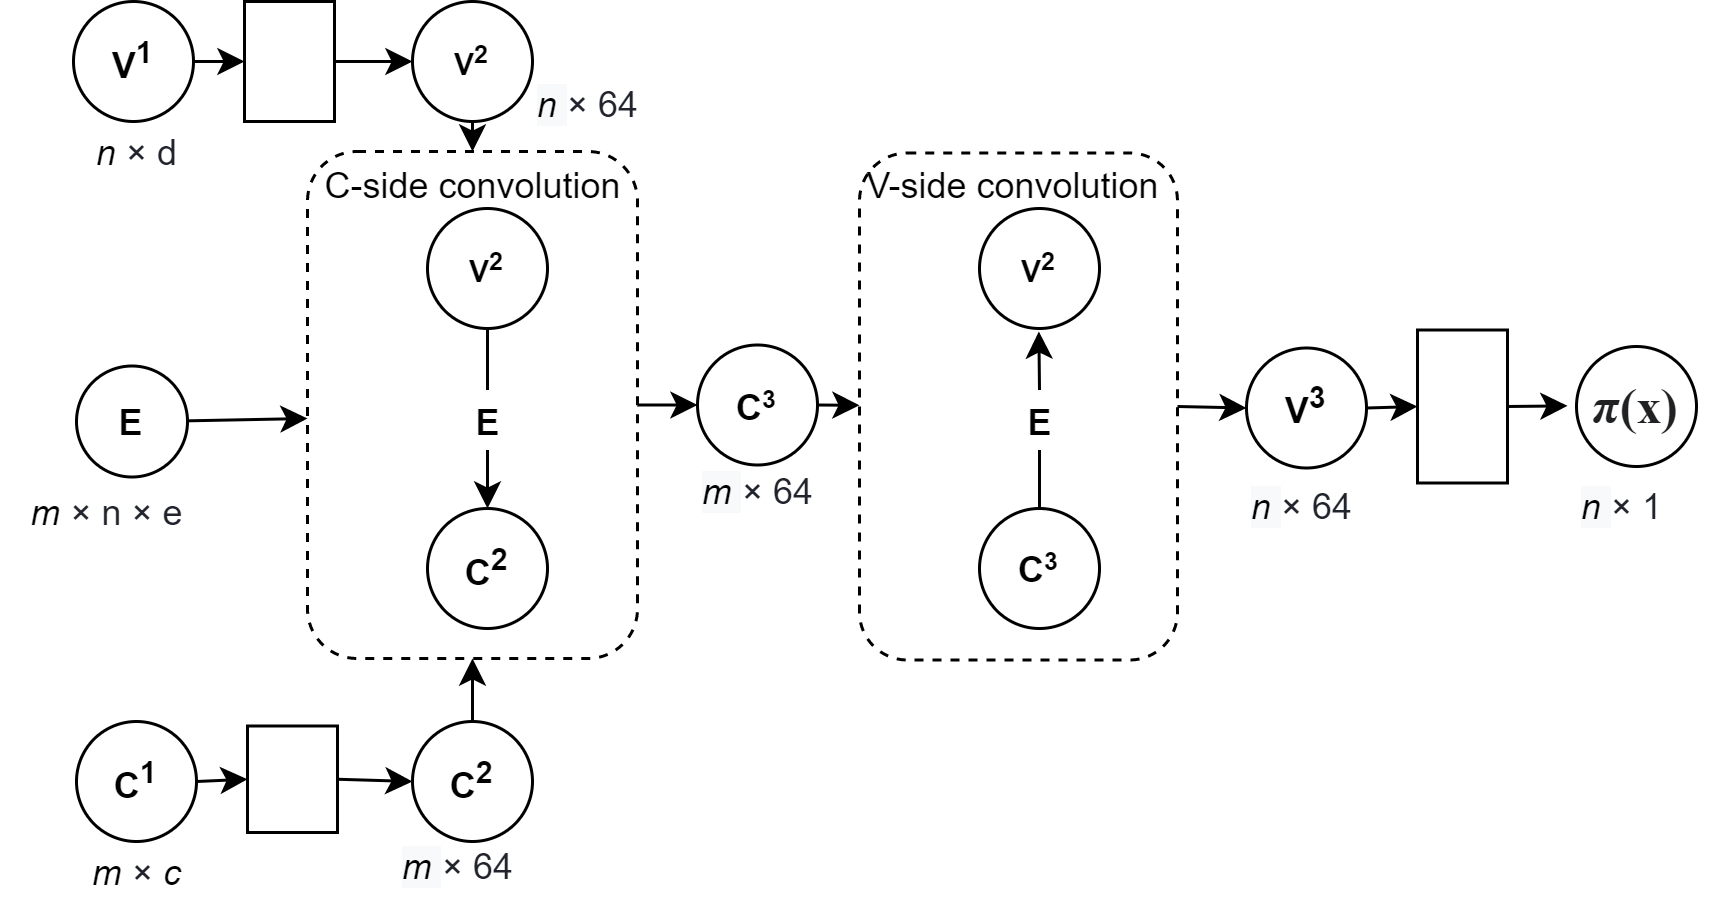
\includegraphics[width=\linewidth]{img/gnn_2.png}
    \caption{The Graph Convolutional Neural Network as specified in Gasse et al. (2019) \cite{gasse2019exact}.}
    \label{fig:gnn2}
\end{figure}






\subsection{Network Topologies}

As stated, the \gls{ML}-models used in the experiments are generated by iteratively ablating (removing components) from the original network. This results in models that are \gls{GCNN}s and models that are pure \gls{MLP}s, which will be compared for accuracy and efficiency on both \gls{GPU} and \gls{CPU}. 

The ablated models are chosen based on three basic assumptions that are assumed to be true based on the vast literature in deep learning \cite{goodfellow2016deep}, and will shown to be correct in the following examples in the thesis\footnote{These assumptions are separate from the three research questions presented in \Cref{sec:int_questions}, and will not be covered in the same detail.}. The assumptions are stated as: 


\begin{enumerate}[label=(\roman*)]
    \item  It is assumed that increasing the capacity of the network correlates to increasing the number of computations \cite{goodfellow2016deep}. 
    \item  It is assumed that the variation in complexity will lead to differences in both accuracy and forward pass computation time \cite{goodfellow2016deep}. 
    \item  It is also assumed that the addition of the graph convolution will be a significant factor in the accuracy and efficiency of the models, particularly on the \gls{CPU}, based on the results in the appendix of Gupta et al. (2020) \cite{gupta2020hybrid}.
\end{enumerate}

Considering this, the experiments will be performed with a total of five models, i.e., the original model and four models stemming from the iterative ablation of this model. Of these, two models will contain the graph convolution operation, and three will be Multi-layer Perceptrons that only use the variable data. 

Results in the specialization project this thesis is based on showed consistent and significant changes in the accuracy-efficiency trade-off were found with a similar selection of \gls{MLP} models, although these models relied on the extended variable feature set developed in Khalil et al. (2016) \cite{khalil2016learning}.

\textit{GNN2}, illustrated in \Cref{fig:gnn1}, is identical (except for the minor, commented details), to the original Gasse \gls{GCNN}.  

\textit{GNN1}, illustrated in \Cref{fig:gnn1}, is the model resulting from the first iteration of the ablation, which has reduced the number of layers in the embeddings and the output module. The graph convolutions are therefore unchanged.

\begin{figure}
    \centering
    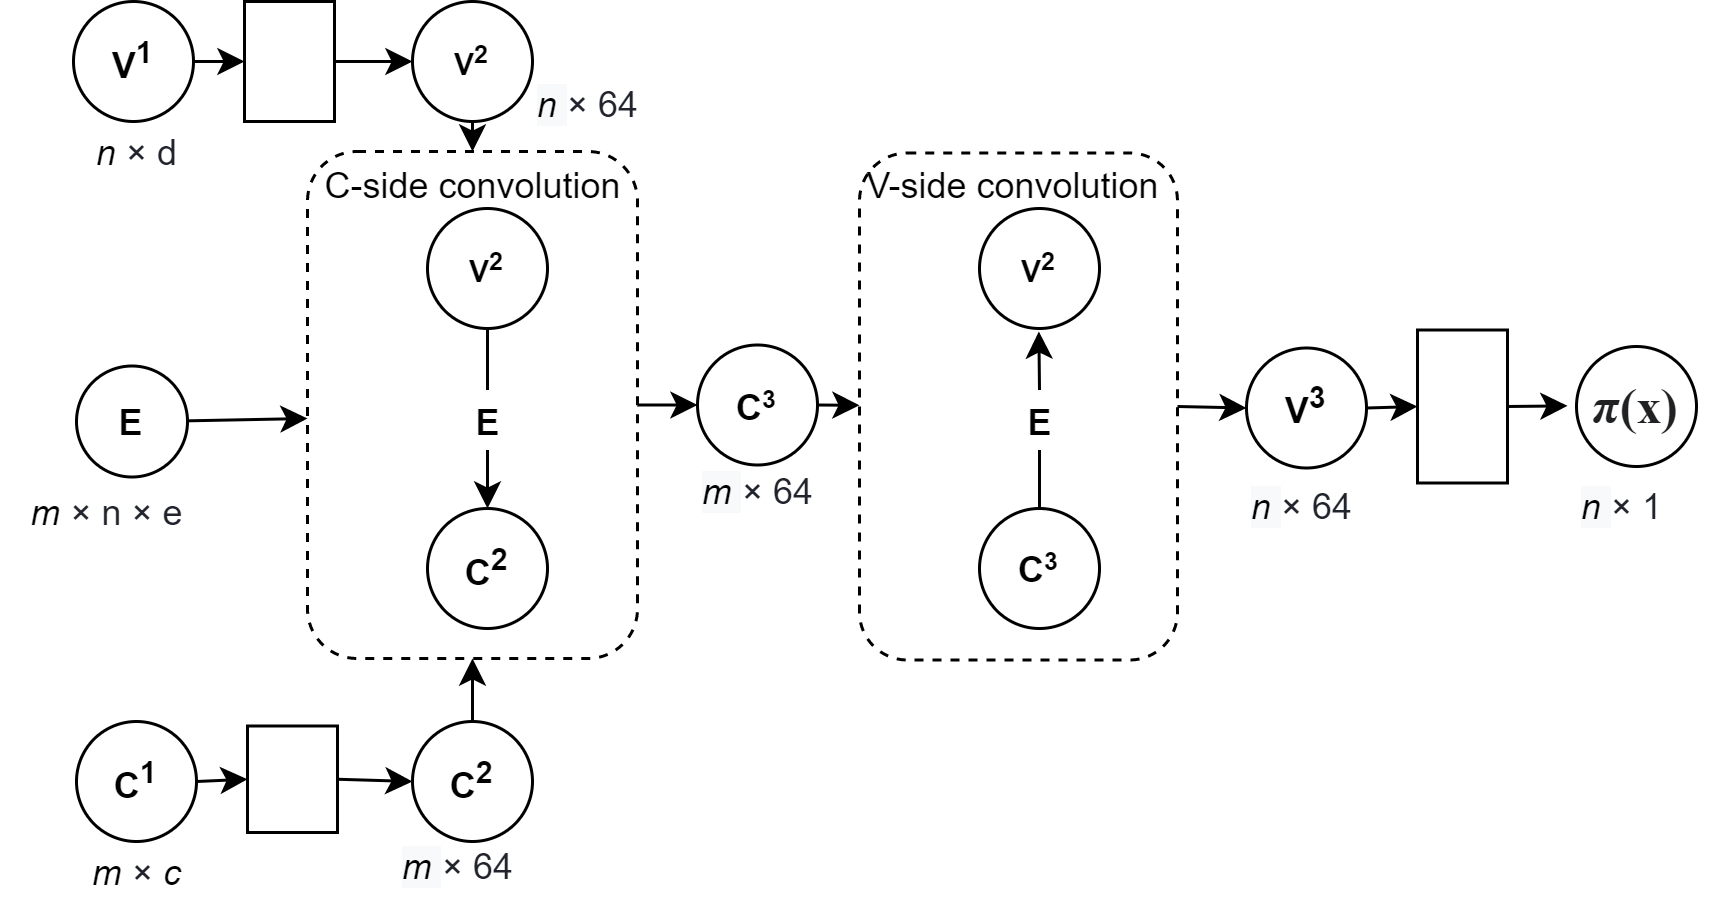
\includegraphics[width=\linewidth]{img/gnn_1.png}
    \caption{The ablated model GNN1.}
    \label{fig:gnn1}
\end{figure}

\textit{\gls{MLP}3} is illustrated in \Cref{fig:topo_mlp3}. The second ablation removes the convolutions in their entirety, resulting in an \gls{MLP} model consisting of the prenorm layer and embedding of the variable features with the output module. This equates to a four-layer \gls{MLP}


\textit{\gls{MLP}2} is illustrated in \Cref{fig:topo_mlp1}. The third ablation removes the prenorm layer and the layers from the MLP3 model, yielding a network with lower capacity but fewer operations needed for evaluation. The two-layer \gls{MLP} also results in a minimal network for representing non-linear relations between the features and the scores. 


\textit{\gls{MLP}1} is illustrated in \Cref{fig:topo_mlp2}. The fourth ablation removes all hidden layers, resulting in an \gls{MLP} model consisting of the prenorm layer and embedding of the variable features with the output module. is equivalent to finding the optimal linear combination of input parameters\footnote{To be exact, MLP1 is not a Multi-Layer Perceptron, however, the name is chosen to be consistent with the other models. The central difference between the models is whether they contain graph convolutions or not (given by the acronym) and the number of parameters (given by the number).}. A forward pass is equivalent to a single matrix multiplication. 


\begin{figure}
    \centering
    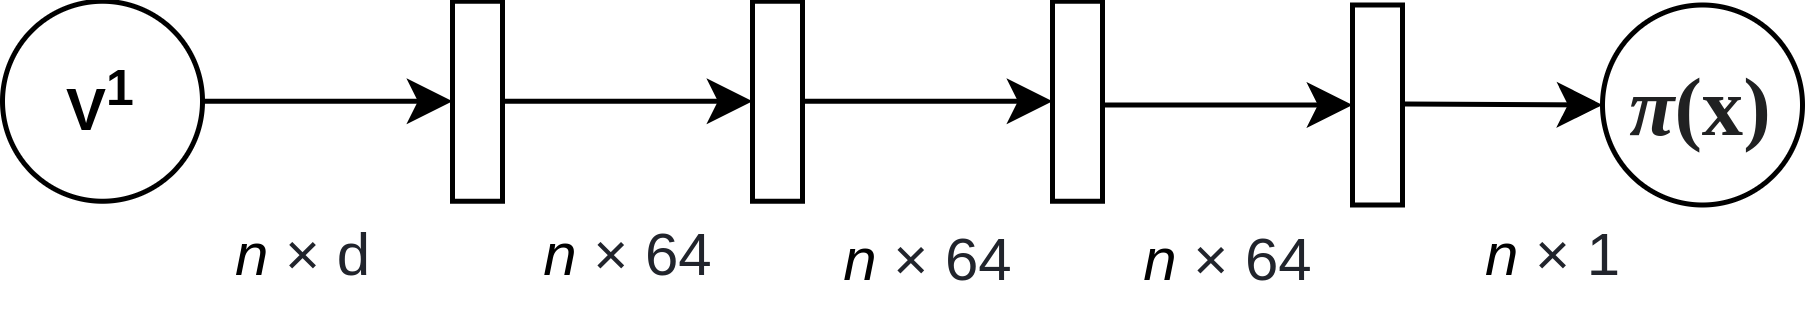
\includegraphics[width=0.7\linewidth]{img/mlp3.png}
    \caption{Topology of the larger sized MLP3 feed-forward network}
    \label{fig:topo_mlp3}
\end{figure}

\begin{figure}
    \centering
    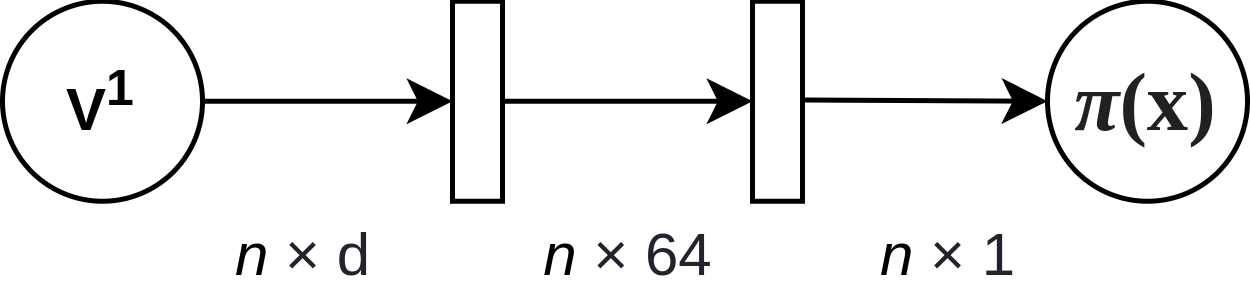
\includegraphics[width=0.6\linewidth]{img/mlp2.png}
    \caption{Topology of the medium sized MLP2 feed-forward network}
    \label{fig:topo_mlp2}
\end{figure}

\begin{figure}
    \centering
    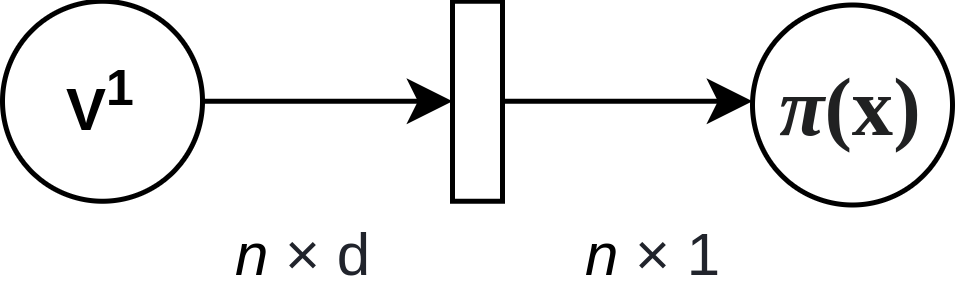
\includegraphics[width=0.5\linewidth]{img/mlp1.png}
    \caption{Topology of the smaller sized MLP1 feed-forward network}
    \label{fig:topo_mlp1}
\end{figure}



\subsection{Network hyperparameters}

All hyperparameters except for the amount and size of the hidden layers is consistent for all models, in order to make a fairer judgment of the accuracy/efficiency trade-off. The activation function is the \textit{Recti-Linear Unit} (ReLU), expressed as $y = \max \{ 0, x\}$. This non-linear activation function is the least computationally expensive of the common activation functions. This is consistent with Gasse et al. (2019) \cite{gasse2019exact} and Gupta et al. (2020) \cite{gupta2020hybrid}.


\section{Training Protocol}\label{sec:trainingprotocol}

In this section, the training protocol is presented, which explains how the parameters of the models are learned.


\subsection{Loss function}

The problem is expressed as a two-class classification problem, where the classes are \textit{optimal variable} and \textit{sub-optimal variable}, respectively. The first class contains only the top variable from the strong branching evaluation. The loss function in binary classification is typically chosen as the binary cross-entropy loss function \cite{goodfellow2016deep}, calculated as:
\begin{align}
    \bm{\mathcal{L}}(\bm{\theta}) &= - \frac{1}{|\mathcal{D}|}\sum_{(\bm{x}, y) \in \mathcal{D}} \left( y_i \cdot \log( \hat y_i) + (1-y_i) \cdot \log(1 - \hat y_i) \right)
\end{align}
This means that for each branching decision, $n$ candidate variables will be given a score analogous to the probability of that variable being the best variable according to the strong branching expert policy. 

\subsection{Training method}

The parameters of the \gls{MLP} are trained via mini-batch gradient descent \cite{goodfellow2016deep}, and is performed using 
 the Adam optimizer \cite{kingma2017adam}. The adam optimizer performs gradient descent with adaptive moments in both the first and second order \cite{kingma2017adam}. 
 The batch size (number of problems processed at once) is set to 32. The learning rate is reduced upon plateaus\footnote{\textit{Plateaus} are multiple epochs without reduction in the target loss.} in validation loss 
 by multiplying with $ 0.2 $. This is a well-known method to ensure convergence to a reasonably good local minimum \cite{goodfellow2016deep}.
 
 Further, the training has implemented an \textit{early stopping scheme}, to ensure that the models have converged, regardless of model complexity. If the validation loss does not decrease 16 epochs in a row, the model that resulted in the lowest validation loss is saved and the training process is stopped. This is because it is considered unlikely for the optimizer to improve the model after that amount of epochs without improvement. 
 
 All of these methods are implemented in order to give the fairest evaluation of the models, as individual hyperparameter optimization for each model would be too time-consuming to be performed. 


\subsection{Computer Hardware}

Training of the \gls{MLP}s is performed on an NVIDIA RTX2070 SUPER GPU (8GB VRAM). The \gls{BnB} solution efficiency evaluations are performed with an Intel i5-2500K \gls{CPU} (4 cores, 6 threads) running at 3.31 GHz. This is less expensive hardware compared to Gasse et al. (2019) \cite{gasse2019exact} and Gupta et al. (2020) \cite{gupta2020hybrid}, particularly the CPU. Variation in processing power is assumed to have an insignificant effect on the relative solution times of the methods, however, \gls{CPU}s with internal acceleration methods for matrix operations might give varying results \cite{vanhoucke2011improving}. It is assumed that the results on the chosen hardware yields a more pessimistic performance overall for the \gls{ML} based methods, and will therefore not be given too much attention in the thesis. Analysis of these differences in hardware and processing performance for both the classical and learned methods on both \gls{CPU} and \gls{GPU} is of interest, but far beyond the scope of this thesis. 



\section{Comparison Method}

The method in which the \gls{MLP}s are compared to each other and the classical branching strategies is presented in this section.


\subsection{Classical Branching Policies}

The accuracy and efficiency of the algorithm with the learned branching rule are evaluated against three branching strategies native to the \gls{SCIP} optimization suite. 

First is the Full Strong Branching (\gls{FSB}) strategy \cite{applegate1995finding}, the slow but accurate expert strategy that performs Strong Branching at every node for every variable. This algorithm is considered of little practical use because of the computationally heavy variable decision process \cite{achterberg2004branching}.

Pseudo-cost Branching (\gls{PC}) is a fast but inaccurate branching strategy \cite{gamrath2018measuring} that chooses the variable that maximizes the lower bound improvement according to the results of previous branching decisions \cite{benchiou1971experiments}. This method does not compute anything for the candidate variables and relies only on previous results. 

Reliability Pseudo-cost Branching (\gls{RPC}) \cite{achterberg2004branching} combines \gls{FSB} and \gls{PC} by performing \gls{SB} on variables with low confidence in the pseudo-costs \cite{gamrath2018measuring}. \gls{RPC} is the default branching strategy in the \gls{SCIP} \gls{BnB} solver. 

The classical variable selection policies will be implemented by configuring the priority of the branching strategies in \gls{SCIP}. 


\subsection{Benchmarking}\label{ssec:benchmarking}

The learned branching strategies are evaluated for both \textit{accuracy} and \textit{efficiency}. 

The accuracy of the strategies is evaluated against the expert decisions of the Full Strong Branching Algorithm. This is done by evaluating the average \textit{top-k accuracy} over an unseen test set. Top-k accuracy measures whether the chosen branching variable was within the top k choices of the Strong Branching algorithm, based on the score given to each candidate variable by the algorithm. Only the \gls{MLP}s are measured in this regard. 

The efficiency of the strategies is evaluated by exchanging the branching strategy of the optimization solver and testing on the data set with three different problem sizes, as described in \Cref{sec:dataset}. For the largest problems, solution time is limited to $ 45 $ minutes, and the number of problems the algorithm does not solve will be reported.
The execution time is compared using python's \verb|time.proc_time()| function, which returns the \gls{CPU} process time \cite{rossum2009python}. 

The number of nodes processed by the algorithm will also be reported. Fewer nodes are not necessarily indicative of a better algorithm, however, this will be an important comparison, as it gives a proxy measurement of the accuracy/efficiency trade-off for the algorithms. 





\section{Software}

A number of comprehensive software libraries are required to perform the experiments in this thesis, this section presents the three most essential.  


\subsection{SCIP}

\textit{Solving Constraint Integer Programs }(\gls{SCIP})
\cite{achterberg2009scip}, is the \gls{CO} solver that lays the foundation for the data generation and model evaluation for the methods. It is considered the fastest non-commercial solver for \gls{MIP} and\gls{MINLP} problems \cite{gamrath2020scip}. It is written in C with wrappers for C++. The software is maintained by the\textit{ Zuse Institute Berlin} (ZIB) group. 

The \textit{SCIP Optimization Suite} contains, as of version 7, the simplex-based linear programming solver SoPlex \cite{wunderling1996soplex}, automated decomposition solver GCG \cite{gamrath2010gcg}, the parallelization framework UG \cite{shinano2018ug} and the \gls{MILP} pre solving library PaPILO \cite{gamrath2020scip}.

In the experiments in this thesis, the LP solver and node selection algorithms are the most relevant, as most of the more complex capabilities of \gls{SCIP} are deactivated in order to make the results as fair and reproducible as possible. 





\subsection{PyTorch}

\textit{PyTorch} is the Python library that the machine learning models are written in. The library provides, most notably, dynamic eager execution, automatic differentiation, and \gls{GPU} acceleration \cite{paszke2019pytorch}. 

Necessary for constructing and training the graph convolutional neural networks, the \textit{PyTorch Geometric} library was used \cite{fey2019pytorchgeometric}. The library facilitates deep learning on data with irregular structures, such as graphs. This includes methods for sparse data GPU acceleration and efficient mini-batch handling \cite{fey2019pytorchgeometric}. 




\subsection{Ecole}\label{ssec:ecole}

To facilitate and standardize the development of \gls{ML}-based improvements of \gls{CO} algorithms, \textit{Extensible Combinatorial Optimization Learning Environments} (\gls{Ecole}) was developed \cite{prouvost2020ecole}, with the first version published in the last quarter of 2020. \gls{Ecole} aims to mimic the \textit{openAI Gym} framework \cite{brockman2016openai}, a popular framework for developing \gls{RL} models. It is a python library written largely in efficient C++. 
The library is based on the open-source solver \gls{SCIP} \cite{achterberg2009scip}.


It also provides \gls{CO} problem \textit{generators} for the four problem classes presented in this thesis. As of version 0.5, these generators are not completely correct, and in the problem generators from Gupta et al. (2020) \cite{gupta2020hybrid} were therefore used. These problems appear to be resolved in version 0.6.  


The theoretical basis for \gls{Ecole} is presented in \Cref{sec:back_mdp}, with the \gls{PO-MDP} formulation relevant for the  
%The relevant functions and their \gls{PO-MDP} counterparts can be presented as follows \cite{prouvost2020ecole}:
%\begin{align*}
%    RewardFunction &\equiv \mathcal{R}\\
%ObservationFunction &\equiv \mathcal{O}\\
%reset\_dynamics() &\equiv p_\textit{init}(s_0)\\
%step\_dynamics() &\equiv p_\textit{trans}(s_{t+1}|s_t,a_t)\\
%reset() &\equiv s_0 \sim p_\textit{init}(s_0), r_0=R(s_0), o_0=O(s_0)\\ 
%step() &\equiv s_{t+1} \sim p_\textit{trans}(s_{t+1}|a_t,s_t)\\ r_t&=R(s_t)\\ o_t&=O(s_t)
%\end{align*}





\subsection{Development Environment}

The project is run on only open-source software, in order to support and further develop the commonly available tools for machine learning and mathematical programming. For reproducibility, the libraries and their respective versions are listed here, as well as in the publicly available code repository. 

The project code is written in 
\verb|python 3.8.5| \cite{rossum2009python}, and uses               
\verb|pytorch 1.6.0| \cite{paszke2019pytorch} for the machine learning models.           

For \gls{GPU} accelerated training, 
\verb|cudnn 7.6.5| and 
\verb|cudatoolkit 10.2.89| \cite{kirk2008nvidia} is used. 

The optimization problems are solved using the \verb|SCIP 7.0.2| Optimization Suite \cite{gamrath2020scip}, using the 
\verb|SoPlex 4.0.1| \cite{wunderling1996soplex} linear programming solver to solve the relaxed problems. The Python interface
\verb|PySCIPOpt 3.0.4| \cite{maher2016pyscipopt} is used in and alongside \gls{Ecole} to facilitate communication with \gls{SCIP}.

The computer is running the \verb|Ubuntu 20.04.2| Linux distribution.


\subsection{Code Repository}

As stated, the code for reproducing the experiments is given in a publicly available code repository, found at \url{https://github.com/Sandbergo/branch2learn}. It is intended to be similar to the source code for Gasse et al. (2019) \cite{gasse2019exact}, and to be extensible in order to facilitate further work. 

A presentation of the code is given in \verb|README.md|, with installation instructions in \verb|INSTALLATION.md|. Installation requires some manual installation but is mostly done using \verb|Anaconda|. The eponymous subdirectory \verb|branch2learn| contains python scripts for running the respective processes of training and evaluating the models: \verb|00_generate_instances.py|, \verb|01_generate_data.py|, \verb|02_train.py|,
\verb|03_test.py|, \\
\verb|04_evaluate.py|, and \verb|05_evaluate_standard.py|.  These are run with parsed arguments. In addition, the directories for the models and utility functions are found there.

The directory \verb|scripts| contains bash-scripts for reproducing all experiments used in this thesis. 